%!TEX encoding = UTF-8 Unicode
\documentclass[french, a4paper, 10pt, twocolumn, landscape]{article}



%% Langue et compilation

\usepackage[utf8]{inputenc}
\usepackage[T1]{fontenc}
\usepackage[french]{babel}
\usepackage{lmodern}       % permet d'avoir certains "fonts" de bonne qualite
\renewcommand{\familydefault}{\sfdefault}
%% LISTE DES PACKAGES

\usepackage{mathtools}     % package de base pour les maths
\usepackage{amsmath}       % mathematical type-setting
\usepackage{amssymb}       % symbols speciaux pour les maths
\usepackage{textcomp}      % symboles speciaux pour el text
\usepackage{gensymb}       % commandes generiques \degree etc...
\usepackage{tikz}          % package graphique
\usepackage{wrapfig}       % pour entourer a cote d'une figure
\usepackage{color}         % package des couleurs
\usepackage{xcolor}        % autre package pour les couleurs
\usepackage{pgfplots}      % pacakge pour creer des graph
\usepackage{epsfig}        % permet d'inclure des graph en .eps
\usepackage{graphicx}      % arguments dans includegraphics
\usepackage{pdfpages}      % permet d'insérer des pages pdf dans le document
\usepackage{subfig}        % permet de creer des sous-figure
% \usepackage{pst-all}       % utile pour certaines figures en pstricks
\usepackage{lipsum}        % package qui permet de faire des essais
\usepackage{array}         % permet de faire des tableaux
\usepackage{multicol}      % plusieurs colonnes sur une page
\usepackage{enumitem}      % pro­vides user con­trol: enumerate, itemize and description
\usepackage{hyperref}      % permet de creer des hyperliens dans le document
\usepackage{lscape}        % permet de mettre une page en mode paysage

\usepackage{fancyhdr}      % Permet de mettre des informations en hau et en bas de page      
\usepackage[framemethod=tikz]{mdframed} % breakable frames and coloured boxes
\usepackage[top=1.8cm, bottom=1.8cm, left=1.5cm, right=1.5cm]{geometry} % donne les marges
\usepackage[font=normalsize, labelfont=bf,labelsep=endash, figurename=Figure]{caption} % permet de changer les legendes des figures
\setlength{\parskip}{0pt}%
\setlength{\parindent}{18pt}
\usepackage{lewis}
\usepackage{bohr}
\usepackage{chemfig}
\usepackage{chemist}
\usepackage{tabularx}
\usepackage{pgf-spectra} % permet de tracer des spectres lumineux des atomes et des ions
\usepackage{pgf}

\usepackage{flexisym}
\usepackage{soul}
\usepackage{ulem}
\usepackage{cancel}

\usepackage{import}
\usepackage{physics}
\usepackage[outline]{contour} % glow around text
\tikzset{every shadow/.style={opacity=1}}


%% LIBRAIRIES

\usetikzlibrary{plotmarks} % librairie pour les graphes
\usetikzlibrary{patterns}  % necessaire pour certaines choses predefinies sur tikz
\usetikzlibrary{shadows}   % ombres des encadres
\usetikzlibrary{backgrounds} % arriere plan des encadres


%% MISE EN PAGE

\pagestyle{fancy}     % Défini le style de la page

\renewcommand{\headrulewidth}{0pt}      % largeur du trait en haut de la page
\fancyhead[L]{\textbf{\textcolor{cyan}{Cours}} - Thème 4 - La Terre un astre singulier}         % info coin haut gauche
\fancyhead[R]{\textit{Première Enseignement Scientifique}}  % info coin haut droit

% % bas de la page
% \renewcommand{\footrulewidth}{0pt}      % largeur du trait en bas de la page
% \fancyfoot[L]{}  % info coin bas gauche
\fancyfoot[R]{Lycée GT Jean Guéhenno}                         % info coin bas droit


\setlength{\columnseprule}{1pt} 
\setlength{\columnsep}{30pt}



%% NOUVELLES COMMANDES 

\DeclareMathOperator{\e}{e} % permet d'ecrire l'exponentielle usuellement


\newcommand{\gap}{\vspace{0.15cm}}   % defini une commande pour sauter des lignes
\renewcommand{\vec}{\overrightarrow} % permet d'avoir une fleche qui recouvre tout le vecteur
\newcommand{\bi}{\begin{itemize}}    % begin itemize
\newcommand{\ei}{\end{itemize}}      % end itemize
\newcommand{\bc}{\begin{center}}     % begin center
\newcommand{\ec}{\end{center}}       % end center
\newcommand\opacity{1}               % opacity 
\pgfsetfillopacity{\opacity}

\newcommand*\Laplace{\mathop{}\!\mathbin\bigtriangleup} % symbole de Laplace

\frenchbsetup{StandardItemLabels=true} % je ne sais plus

\newcommand{\smallO}[1]{\ensuremath{\mathop{}\mathopen{}o\mathopen{}\left(#1\right)}} % petit o

\newcommand{\cit}{\color{blue}\cite} % permet d'avoir les citations de couleur bleues
\newcommand{\bib}{\color{black}\bibitem} % paragraphe biblio en noir et blanc
\newcommand{\bthebiblio}{\color{black} \begin{thebibliography}} % idem necessaire sinon bug a cause de la couleur
\newcommand{\ethebiblio}{\color{black} \end{thebibliography}}   % idem
%%% TIKZ


%% COULEURS 


\definecolor{definitionf}{RGB}{220,252,220}
\definecolor{definitionl}{RGB}{39,123,69}
\definecolor{definitiono}{RGB}{72,148,101}

\definecolor{propositionf}{RGB}{255,216,218}
\definecolor{propositionl}{RGB}{38,38,38}
\definecolor{propositiono}{RGB}{109,109,109}

\definecolor{theof}{RGB}{255,216,218}
\definecolor{theol}{RGB}{160,0,4}
\definecolor{theoo}{RGB}{221,65,100}

\definecolor{avertl}{RGB}{163,92,0}
\definecolor{averto}{RGB}{255,144,0}

\definecolor{histf}{RGB}{241,238,193}

\definecolor{metf}{RGB}{220,230,240}
\definecolor{metl}{RGB}{56,110,165}
\definecolor{meto}{RGB}{109,109,109}


\definecolor{remf}{RGB}{230,240,250}
\definecolor{remo}{RGB}{150,150,150}

\definecolor{exef}{RGB}{240,240,240}

\definecolor{protf}{RGB}{247,228,255}
\definecolor{protl}{RGB}{105,0,203}
\definecolor{proto}{RGB}{174,88,255}

\definecolor{grid}{RGB}{180,180,180}

\definecolor{titref}{RGB}{230,230,230}

\definecolor{vert}{RGB}{23,200,23}

\definecolor{violet}{RGB}{180,0,200}

\definecolor{copper}{RGB}{217, 144, 88}

%% Couleur des ref

\hypersetup{
	colorlinks=true,
	linkcolor=black,
	citecolor=blue,
	urlcolor=black
		   }

%% CADRES

\tikzset{every shadow/.style={opacity=1}}

\global\mdfdefinestyle{doc}{backgroundcolor=white, shadow=true, shadowcolor=propositiono, linewidth=1pt, linecolor=black, shadowsize=5pt}
\global\mdfdefinestyle{titr}{backgroundcolor=metf, shadow=true, shadowcolor=propositiono, linewidth=1pt, linecolor=black, shadowsize=5pt}
\global\mdfdefinestyle{theo}{backgroundcolor=theof, shadow=true, shadowcolor=theoo, linewidth=1pt, linecolor=theol, shadowsize=5pt}
\global\mdfdefinestyle{prop}{backgroundcolor=theof, shadow=true, shadowcolor=propositiono, linewidth=1pt, linecolor=theol, shadowsize=5pt}
\global\mdfdefinestyle{def}{backgroundcolor=definitionf, shadow=true, shadowcolor=definitiono, linewidth=1pt, linecolor=definitionl, shadowsize=5pt}
\global\mdfdefinestyle{histo}{backgroundcolor=histf, shadow=true, shadowcolor=propositiono, linewidth=1pt, linecolor=black, shadowsize=5pt}
\global\mdfdefinestyle{avert}{backgroundcolor=white, shadow=true, shadowcolor=averto, linewidth=1pt, linecolor=avertl, shadowsize=5pt}
\global\mdfdefinestyle{met}{backgroundcolor=metf, shadow=true, shadowcolor=meto, linewidth=1pt, linecolor=metl, shadowsize=5pt}
\global\mdfdefinestyle{rem}{backgroundcolor=metf, shadow=true, shadowcolor=meto, linewidth=1pt, linecolor=metf, shadowsize=5pt}
\global\mdfdefinestyle{exo}{backgroundcolor=exef, shadow=true, shadowcolor=propositiono, linewidth=1pt, linecolor=exef, shadowsize=5pt}
\global\mdfdefinestyle{not}{backgroundcolor=definitionf, shadow=true, shadowcolor=propositiono, linewidth=1pt, linecolor=black, shadowsize=5pt}
\global\mdfdefinestyle{proto}{backgroundcolor=protf, shadow=true, shadowcolor=proto, linewidth=1pt, linecolor=protl, shadowsize=5pt}

%%%%%%
\definecolor{cobalt}{rgb}{0.0, 0.28, 0.67}
\definecolor{applegreen}{rgb}{0.55, 0.71, 0.0}

\usepackage{tcolorbox}
  \tcbuselibrary{most}
  \tcbset{colback=cobalt!5!white,colframe=cobalt!75!black}



\newtcolorbox{definition}[1]{
	colback=applegreen!5!white,
  	colframe=applegreen!65!black,
	fonttitle=\bfseries,
  	title={#1}}
\newtcolorbox{Programme}[1]{
	colback=cobalt!5!white,
  	colframe=cobalt!65!black,
	fonttitle=\bfseries,
  	title={#1}} 
\newtcolorbox{Proposition}[1]{
      colback=theof,%!5!white,
        colframe=theol,%!65!black,
      fonttitle=\bfseries,
        title={#1}}  

\newtcolorbox{Exercice}[1]{
  colback=cobalt!5!white,
  colframe=cobalt!65!black,
  fonttitle=\bfseries,
  title={#1}}  

\newtcolorbox{Resultat}[1]{
	colback=theof,%!5!white,
	colframe=theoo!85!black,
  fonttitle=\bfseries,
	title={#1}} 	

  \setlength{\tabcolsep}{20pt}

  \renewcommand{\arraystretch}{1.5}
  
  \newcommand{\pisteverte}{
	\begin{flushleft}
		\begin{tikzpicture}
			\draw (0,0) -- (0,.2);
			\draw[fill = green] (0,0.4) circle (0.2);
			\node[draw] at (1.5,0.3) {Piste verte};
		\end{tikzpicture}
		\end{flushleft}
}

\newcommand{\pistebleue}{
	\begin{flushleft}
		\begin{tikzpicture}
			\draw (0,0) -- (0,.2);
			\draw[fill = blue] (0,0.4) circle (0.2);
			\node[draw] at (1.5,0.3) {Piste bleue};
		\end{tikzpicture}
		\end{flushleft}
}
\newcommand{\pistenoire}{
	\begin{flushleft}
		\begin{tikzpicture}
			\draw (0,0) -- (0,.2);
			\draw[fill = black!80] (0,0.4) circle (0.2);
			\node[draw] at (1.5,0.3) {Piste noire};
		\end{tikzpicture}
		\end{flushleft}
}
  \newcommand{\titre}[1]{
    \begin{mdframed}[style=titr, leftmargin=0pt, rightmargin=0pt, innertopmargin=8pt, innerbottommargin=8pt, innerrightmargin=10pt, innerleftmargin=10pt]
      \begin{center}
        \Large{\textbf{#1}}
      \end{center}
    \end{mdframed}
  }


  %% COMMANDE Exercice
  
  \newcommand{\exo}[3]{
    \begin{mdframed}[style=exo, leftmargin=0pt, rightmargin=0pt, innertopmargin=8pt, innerbottommargin=8pt, innerrightmargin=10pt, innerleftmargin=10pt]
  
      \noindent \textbf{Exercice #1 - #2}\medskip
  
      #3
    \end{mdframed}
  }
  
     
  \newcommand{\questions}[1]{
    \begin{mdframed}[style=exo, leftmargin=0pt, rightmargin=0pt, innertopmargin=8pt, innerbottommargin=8pt, innerrightmargin=10pt, innerleftmargin=10pt]
  
      \noindent \textbf{Questions :}\smallskip
  
      #1
    \end{mdframed}
  }
  
  \newcommand{\doc}[3]{
    \begin{mdframed}[style=doc, leftmargin=0pt, rightmargin=0pt, innertopmargin=8pt, innerbottommargin=8pt, innerrightmargin=10pt, innerleftmargin=10pt]
  
      \noindent \textbf{Document #1 - #2}\medskip
  
      #3
    \end{mdframed}
  }
\def\width{12}
\def\hauteur{5}


\usetikzlibrary{intersections}
\usetikzlibrary{decorations.markings}
\usetikzlibrary{angles,quotes} % for pic
\usetikzlibrary{calc}
\usetikzlibrary{3d}
\contourlength{1.3pt}

\tikzset{>=latex} % for LaTeX arrow head
\colorlet{myred}{red!85!black}
\colorlet{myblue}{blue!80!black}
\colorlet{mycyan}{cyan!80!black}
\colorlet{mygreen}{green!70!black}
\colorlet{myorange}{orange!90!black!80}
\colorlet{mypurple}{red!50!blue!90!black!80}
\colorlet{mydarkred}{myred!80!black}
\colorlet{mydarkblue}{myblue!80!black}
\tikzstyle{xline}=[myblue,thick]
\def\tick#1#2{\draw[thick] (#1) ++ (#2:0.1) --++ (#2-180:0.2)}
\tikzstyle{myarr}=[myblue!50,-{Latex[length=3,width=2]}]
\def\N{90}

\tikzset{
  % style to apply some styles to each segment of a path
  on each segment/.style={
    decorate,
    decoration={
      show path construction,
      moveto code={},
      lineto code={
        \path [#1]
        (\tikzinputsegmentfirst) -- (\tikzinputsegmentlast);
      },
      curveto code={
        \path [#1] (\tikzinputsegmentfirst)
        .. controls
        (\tikzinputsegmentsupporta) and (\tikzinputsegmentsupportb)
        ..
        (\tikzinputsegmentlast);
      },
      closepath code={
        \path [#1]
        (\tikzinputsegmentfirst) -- (\tikzinputsegmentlast);
      },
    },
  },
  % style to add an arrow in the middle of a path
  mid arrow/.style={postaction={decorate,decoration={
        markings,
        mark=at position .5 with {\arrow[#1]{stealth}}
      }}},
}



\usetikzlibrary{3d, shapes.multipart}

% Styles
\tikzset{>=latex} % for LaTeX arrow head
\tikzset{axis/.style={black, thick,->}}
\tikzset{vector/.style={>=stealth,->}}
\tikzset{every text node part/.style={align=center}}
\usepackage{amsmath} % for \text
 
\usetikzlibrary{decorations.pathreplacing,decorations.markings}

%% MODIFICATION DE CHAPTER  
\makeatletter
\def\@makechapterhead#1{%
  %%%%\vspace*{50\p@}% %%% removed!
  {\parindent \z@ \raggedright \normalfont
    \ifnum \c@secnumdepth >\m@ne
        \huge\bfseries \@chapapp\space \thechapter
        \par\nobreak
        \vskip 20\p@
    \fi
    \interlinepenalty\@M
    \Huge \bfseries #1\par\nobreak
    \vskip 40\p@
  }}
\def\@makeschapterhead#1{%
  %%%%%\vspace*{50\p@}% %%% removed!
  {\parindent \z@ \raggedright
    \normalfont
    \interlinepenalty\@M
    \Huge \bfseries  #1\par\nobreak
    \vskip 40\p@
  }}
  
  \newcommand{\isotope}[3]{%
     \settowidth\@tempdimb{\ensuremath{\scriptstyle#1}}%
     \settowidth\@tempdimc{\ensuremath{\scriptstyle#2}}%
     \ifnum\@tempdimb>\@tempdimc%
         \setlength{\@tempdima}{\@tempdimb}%
     \else%
         \setlength{\@tempdima}{\@tempdimc}%
     \fi%
    \begingroup%
    \ensuremath{^{\makebox[\@tempdima][r]{\ensuremath{\scriptstyle#1}}}_{\makebox[\@tempdima][r]{\ensuremath{\scriptstyle#2}}}\text{#3}}%
    \endgroup%
  }%

\makeatother


\definecolor{darkpastelgreen}{rgb}{0.01, 0.75, 0.24}
\newcommand{\mobiliser}{
  % \begin{flushleft}
    \begin{tikzpicture}[scale=0.6]
      % \draw (0,0) -- (0,.2);
      \draw[color = darkpastelgreen, fill = darkpastelgreen] (0,-0.3) circle (0.3)node[white]{M};
      % \node[draw, white] at (0,-0.3) {\textbf{M}};
    \end{tikzpicture}
    % \end{flushleft}
}

\newcommand{\realiser}{
  % \begin{flushleft}
    \begin{tikzpicture}[scale=.6]
      % \draw (0,0) -- (0,.2);
      \draw[color = blue, fill = blue] (0,-0.3) circle (0.3) node[white]{R};
      % \node[draw, white] at (0,-0.3) {\textbf{R}};
    \end{tikzpicture}
    % \end{flushleft}
}

\definecolor{bostonuniversityred}{rgb}{0.8, 0.0, 0.0}

\newcommand{\analyser}{
  % \begin{flushleft}
    \begin{tikzpicture}[scale=.6]
      % \draw (0,0) -- (0,.2);
      \draw[color = bostonuniversityred, fill = bostonuniversityred] (0,-0.3) circle (0.3) node[white]{A};
      % \node[draw, white] at (0,-0.3) {\textbf{A}};
    \end{tikzpicture}
    % \end{flushleft}
}
\definecolor{amethyst}{rgb}{0.6, 0.4, 0.8}

\newcommand{\communiquer}{
  % \begin{flushleft}
    \begin{tikzpicture}[scale=.6]
      % \draw (0,0) -- (0,.2);
      \draw[color = amethyst, fill = amethyst] (0,-0.3) circle (0.3) node[white]{C};
      % \node[draw, white] at (0,-0.3) {\textbf{C}};
    \end{tikzpicture}
    % \end{flushleft}
}

\newcommand{\applicationnumerique}{\textbf{A.N.:}}

\usepackage{esint}
\usepackage{breqn}
\usepackage{colortbl}
\newcommand{\objectifs}[1]{
	\begin{minipage}{.02\textheight}
	\rotatebox{90}{\textbf{\large Objectifs}}
	\end{minipage}
	\begin{minipage}{.9\linewidth}
			#1 
	\end{minipage}
}
%%
%%
%% DEBUT DU DOCUMENT
%%

\begin{document}
\section*{Leçon 9: Conversion de puissance électromécanique}

\hrulefill\\
	\underline{Niveau:}
	\begin{itemize}
		\item CPGE PSI
	\end{itemize}
	\underline{Pré-requis:} 
	\begin{itemize}
        \item Electromagnetisme
		\item Mécanique
	\end{itemize}
	\uline{Bibliographie:}
	\begin{itemize}
		%\item BFR \textit{Optique, Chap 10}
		%\item Pérez \textit{Optique}
		\item Physique expérimentale, Jolidon
		\item Cours Naval Conversion électro-magneto-mécanique
		\item Dunod PSI
		\item Physique Chimie en PSI/PSI*, chez ellipses par Pascal Olive
		%\item \url{https://phyanim.sciences.univ-nantes.fr/Ondes/lumiere/interference_lumiere.php}
	\end{itemize}
\hrulefill

\section*{Introduction}
Le phénomène d’induction électromagnétique a mis en évidence la possibilité
de convertir de l’énergie électrique en énergie mécanique et réciproquement. Ce phénomène est souvent illustré par l'exemple du rail de Laplace, où une tige conductrice parcourue par un courant se met en mouvement sous l'action d'un champ magnétique\medskip

L’étude d’une machine électromécanique nécessite de connaître l’expression de
la force (translation) ou du couple (rotation) s’exerçant sur la partie mobile. Les
machines réelles sont constituées de matériaux ferromagnétique, le calcul direct des
actions électromécaniques n’est alors pas envisageable. On choisit une présentation énergétique, plus générale de la conversion électromamécanique.\medskip

Parler des systèmes mettant en \oe uvre le couplage entre induction (loi de Faraday) et les forces de Lorentz. \medskip

Présenter le contacteur électromagnétique puis Machine synchrone et enfin Moteur à courant continu en suivant le programme qui fait systématiquement l'analogie entre sychrone et MCC pour donner l'expression du couple. C'est ambitieux niveau temps surtout avec la mesure du couple pour le moteur à courant continu...

\section*{1. Contacteur électromagnétique en translation}

\subsection*{1.1. Principe de fonctionnement (Dunod PSI + cours naval)}

On considère un noyau ferromagnétique fixe en forme de U, excité par une bobine de $N$ spires parcourue par un couant d'intensité $i$. Deux entrefers d'épaisseur $x$ variable le séparent d'un bloc ferromagnétique mobile en translation selon $Ox$, qu'on appelle \og{}contacteur électromagnétique\fg{}\medskip
On dessine le schéma du système et on procède par étapes:

\begin{figure}[ht]
    \centering
    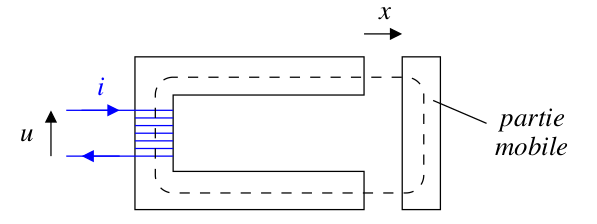
\includegraphics[width=.5\linewidth]{./figures/ContacteurElectromagnetique.png}
    \caption{Contacteur électromagnétique}
\end{figure} 

On considère le matériau  ferromagnétique comme linéaire $\mu_r\ll 1$. Il canalise les lignes de champ magnétique (on peut montrer une simulation PSI Dunod (2020)). On supposera aussi que la section du noyau est petite de façon à ce que $\vec{B}$ et \vec{H} soient uniformes dans une section droite du fer. On note $l$ la longueur moyenne en l'absence de l'entrefer. Si $x$ est suffisamment petit devant $\sqrt{Section}$, le tube de champ magnétique est de section constante dans l'entrefer.

\subsection*{1.2. Énergie magnétique emmagasinée}
\begin{enumerate}
    \item Théorême d'Ampère);

Application du théorême d'Ampère (dans l'ARQS) sur le contour en pointillé: 
\begin{equation}
	H_{fer}\times l + H_{entrefer}\times 2x = Ni
\end{equation}
	\item Conservation du flux du champ magnétique;
	
\begin{equation}
	B_{fer}=B_{entrefer}=B
\end{equation}

    \item Expression de \vec{B} en fonction de l'intensité;

$B_{entrefer}=\mu_0 H_{entrefer}$ et $B_{fer} = \mu_0\mu_rH_{fer}$ En combinant les différentes relations, on en déduit: 
\begin{equation}
	\dfrac{Bl}{\mu_0\mu_r}+\dfrac{B2x}{\mu_0}=Ni\ \rightarrow B = \dfrac{\mu_0Ni}{2x+l/\mu_r}
\end{equation}

    \item Induction propre $\Phi=Li$ à partir du flux dans le bobinage $\Phi=NBS$.

On en déduit : $\Phi = \dfrac{\mu_0N^2S}{2x+l/\mu_r}i$ puis l'expression de $L$.
\begin{equation}
	L(x)=\dfrac{\mu_0N^2S}{2x+l/\mu_r}
\end{equation}
On remarque que dans un circuit magnétique linéaire déformable, l'inductance dépend de la position de la partie mobile.

    \item Énergie magnétique emmagasinée.
\end{enumerate}
\begin{equation}
	E_m = \dfrac{1}{2}L(x)i^2 = \dfrac{1}{2}\dfrac{\mu_0N^2S}{2x+l/\mu_r}i^2.
\end{equation}

Remarque: On peut retrouver ce résultat en utilisant l'expression de l'énergie magnétique volumique : $u_m=B^2/(2\mu_0\mu_r)$ dans un matériau LHI.

\subsection*{1.3. Force électromagnétique (PSI Tec $\&$ Doc 2014)}
On considère l'ensemble constitué par la bobine, les ferromagnétiques et l'entrefer. On suppose qu’un opérateur extérieur déplace le barreau en exerçant la force $\vec{F}_{op}=F_{op}\vec{u}_x$, la bobine
étant traversée par un courant i et soumise à la tension u.

\begin{figure}[ht]
	\centering
	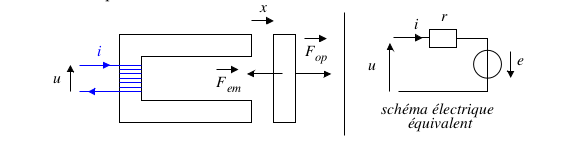
\includegraphics[width=.5\linewidth]{./figures/ForceElectromagnetique.png}
	\caption{Schéma équivalent}
\end{figure}

\subsubsection*{1.3.1. Équation électrique:}
\begin{equation}
	u = ri -e = ri +\dfrac{d\Phi}{dt} \label{eq:eq1CElectromeca}
\end{equation}

\subsubsection*{1.3.2. Premier principe: }
Pendant $dt$, le système reçoit une énergie électrique ($uidt$) et une énergie mécanique $F_{op}dx$ sous forme de travail de la force extérieur qui s'applique sur le bloc en translation. Une partie de l'énergie est dissipée par effet Joule ($Ri^2dt$).
\begin{equation}
	d(E_m+E_c) = \delta W + \delta Q = (uidt+F_{op}dx)-ri^2dt
\end{equation}

Avec l'équation \eqref{eq:eq1CElectromeca} on obtient : 
\begin{equation}
	d(E_m+E_c) = id \Phi+F_{op}dx \label{eq:eq2CElectromeca}
\end{equation}

\subsubsection*{1.3.3. Théorême de l'énergie cinétique (appliqué à la partie mobile)}
\begin{equation}
	dE_c=F_{op}dx+F_{m}dx \label{eq:eq3CElectromeca}
\end{equation}

On compare les équations \eqref{eq:eq2CElectromeca} et \eqref{eq:eq3CElectromeca}, ce qui donne: 
\begin{equation}
	dE_m = id\Phi-F_{m}dx \rightarrow F_{m}dx = id(Li)-d(\dfrac{1}{2}Li^2) \label{eq:eq4CElectromeca}
\end{equation}

Si on développe on trouve : $F_{m}= \dfrac{1}{2}i^2\dfrac{dL}{dx}$ soit:
\begin{equation}
	F_{m} = -\dfrac{\mu_0N^2Si^2}{\left(l/\mu_r+2x\right)^2}
\end{equation}

Si on prend pour valeur $\mu_r=2000$, $N = 500$, $l=50~\rm cm$, $S=16~\rm cm^2$ avec un courant sinusoïdal à $50$ Hz et d'amplitude 50 mA. On trouve $F = 10$ N. On peut lever une masse de 1 kg avec ce dispositif. 

\begin{Resultat}{Il faut noter que :}
	\begin{itemize}
		\item $F_{m}\propto i^2$, c'est une force de rappel quelque soit le signe de $i$ et est nulle en moyenne dans le temps pour une excitation sinusoïdale.
		\item Ce type de dispositif peut servir de contacteur électromagnétique permettant de commander la fermeture et l'ouverture d'un circuit électrique via le déplacement de la partie mobile, qui en l'absence de courant dans la bobine, est ramenée à sa position initiale par l'intermédiaire d'un ressort.
		(\textbf{Discussion et ordre de grandeur} dans le Physique Chimie en PSI/PSI*, chez ellipses par Pascal Olive)
	\end{itemize}
\end{Resultat}

\subsection*{1.4. Généralisation}
La méthode que l'on a appliqué sera toujours la même (Ampère, conservation du flux, inductance propre, énergie emmagasinée, bilan énergétique global). On peut généraliser l'expression de la Force à partir de l'équation \eqref{eq:eq4CElectromeca} tel que : 
\begin{equation}
    F=\left(\dfrac{\partial E}{\partial x}\right)_\Phi
\end{equation}
Pour un contacteur en rotation autour d'un axe fixe $Oz$ repéré par un angle $\theta$, il suffit de changer les travaux extérieurs $\vec{F}_{op}$ et électromagnétique $F_{em}$ en $\Gamma_{op}d\theta$ et $\Gamma_{em}d\theta$ où les $\Gamma$ sont les moments des actions s'exerçant sur le contacteur. 
\begin{equation}
 \Gamma = \left(\dfrac{\partial E}{\partial\theta}\right)_\Phi
\end{equation}



On peut maintenant traité les différents types de moteur. Au programme de PSI ils traient les moteurs synchrones puis à courant continu. La manipulation porte sur un moteur à courant continu donc je choisis de commencer par un moteur à courant continu. On garde néanmoins le moteur synchrone sous le coude pour une troisième partie si le temps le permet (j'en doute) ou pour une ouverture.


\section*{2. Machine à courant continu}
On a vu en première année de PTSI le principe d'action d'un champ magnétique tournant sur un moment magnétique. On réalise la mise en pratique d'un moteur.\medskip

Les machines à courant continu font partie des convertisseurs électro-magnéto-mécanique réversibles. Elles sont utilisées massivement dans toutes les gammes de puissance du fait de la simplicité de leur commande de vitesse.

\subsection*{2.1. Structure}

Les élements qui constituent une machine à courant continu sont: 
\begin{itemize}
	\item Une partie fixe: \textbf{le stator}. Ferro. aimantation permanente ou bobinage parcouru par un courant continu $i_e$. présenté sur le schéma avec une paire de pôle (N et S). Le stator crée un champ magnétique stationnaire $\vec{B}_s$ canalisé par le ferro. Le champ statorique est radial dans l'entrefer.
	
	\item une partie mobile: \textbf{le rotor}. Tourne autour de l'axe $Oz$, ferromagnétique. Encoches incrustées dans le rotor dans lesquelles se logent des conducteurs appelés \og{}brins\fg{}. Ces conducteurs sont disposés en spires bobinées sur le rotor. Les spires sont en série et sont parcourues par le même courant $i$. Le rotor est le siège d'induction de Lorentz.
	
	\item L'organisation des courants rotoriques doit être agencée afin de produire un axe polaire fixe, dirigé de préférence selon $Oy$ pour que le couple soit maximal. Cette propriété est vérifiée si la répartition des courants admet, malgré la rotation du rotor, un plan d'antisymétrie ($Oyz$). Il faut aménager un dispositif qui permet d'imposer un sens de circulation du courant pour la part du bobinage située d'un côté de ce plan et d'inverser ce sens pour celle située de l'autre côté. Ce dispositif se nomme le \textbf{collecteur}. Les spires sont connectées au circuit extérieur par l'intermédiaire des lames du collecteur sur lesquelles frottent les balais. On explique plus en détail le fonctionnement dans la section suivante !
\end{itemize}
\begin{figure}[ht]
	\centering
	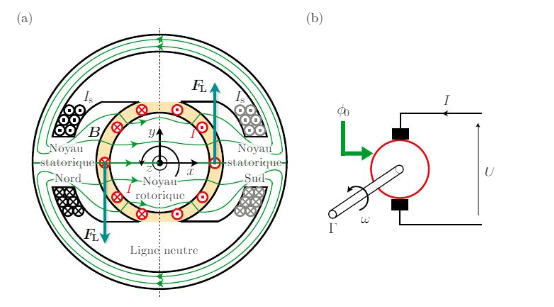
\includegraphics[width=.5\linewidth]{./figures/StructureMCC.png}
	\caption{Schéma d'une machine à courant continu (MCC). Physique Chimie PSI P.Olive, p721. On peut aussi rajouter la simulation des lignes de champ présente dans le Dunod de PSI.}
\end{figure}

\subsection*{2.2. Rôle du collecteur}

Le circuit induit (rotor) est alimenté par le courant continu $i$ qui entre dans le circuit par le pôle + de l'alimentation externe. Une des spires est repérée par la position $\theta$. La connexion de cette spire au circuit d'alimentation montre que si cette connexion reste fixe, le sens de circulation du courant pour la partie de la spire située à gauche du plan $Oyz$ s'inverserait périodiquement en fonction de $\theta$ avec une période de $\pi$.Pour éviter ce changement de sens, on connecte les spires du rotor à l'alimentation par l'intermédiaire d'un collecteur, fixé au sommet du rotor qui permet de raccorder, selon la position de la spire, les bornes de l'alimentation à des extrémités différentes de la spire.\medskip
\begin{figure}[ht]
	\centering
	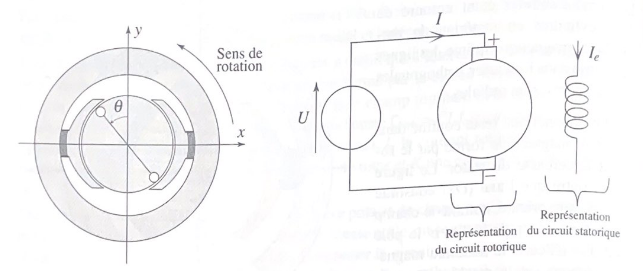
\includegraphics[width=.5\linewidth]{./figures/collecteur1.png}
	\caption{Dunod Psi p 784}
\end{figure}
Le collecteur comporte un ensemble de lames conductrices, électriquement isolées entre elles, situées en tête du rotor. Leur nombre dépend du nombre de spires. L'ensemble de ces lames sont positionnées sur un cylindre posé sur le rotor. Elles tournent donc à la même vitesse que le rotor. Lorsqu'il n'y a qu'une seule spire, le collecteur est composé de deux lames uniquement.

\begin{figure}[ht]
	\centering
	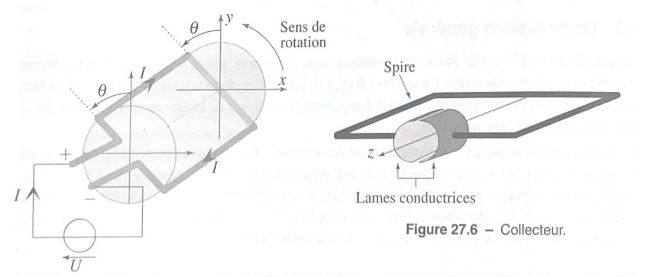
\includegraphics[width=.5\linewidth]{./figures/collecteur2.png}
	\caption{Dunod Psi p 784}
\end{figure}

Le contact entre les lames et le générateur qui alimente le circuit est assuré par deux patins conducteurs fixes (liés au stator), glissant sur les lames du collecteur qui se nomment balais. Lorsque le collecteur tourne avec le rotor, les balais sont au contact de lames différentes. 

\begin{figure}[ht]
	\centering
	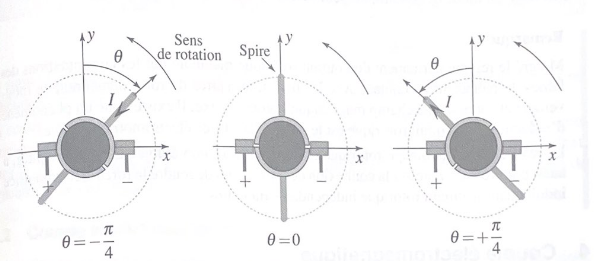
\includegraphics[width=.5\linewidth]{./figures/collecteur3.png}
	\caption{Dunod Psi p 784}
\end{figure}

Pour une seule spire, la direction de l'axe polaire oscille au cours de la rotation du rotor entre $-\pi/2$ et $\pi/2$. Cette oscillation est éliminer dès lors que l'on met un grand nombre de spires. On maintient ainsi la répartition des courants admettant le plan ($Oyz$) comme plan d'antisymétrie. Le champ magnétique est permanent et admet $(Oy)$ comme axe polaire orthogonal à l'axe polaire du stator. Son sens dépend du signe de l'intensité $i$ et du mode de fonctionnement moteur ou générateur de la machine.


\subsection*{2.3. Aproche théorique (Jolidon p 204)}

\subsubsection*{Établissement des équations électromécaniques}

La forme du circuit magnétique cinstitué par le stator et le rotor permet d'établir dans l'entrefer un champ radial. On considère une spire rotorique de hauteur $l$ selon $Oz$ et de largeur $a$, on note I le courant y circulant qui parcourt le segment en $x>0$ selon les $z$ croissants. Le rotor est plongé dans le champ magnétique statorique, chaque segment de spire est parcouru par le courant $I$ subit une force de Laplace:


\begin{equation}
	 d\vec{F}_L =  Idz\vec{e_z}\wedge B\vec{er} = IBdz\vec{e}_\theta
\end{equation}

Cette force est égale à celle s'exerçant sur un point de la spire parallèle à l'axe Oz. Elle génère un couple sur le rotor appelé couple de Laplace. Calculons ce couple.

\begin{figure}[ht]
	\centering
	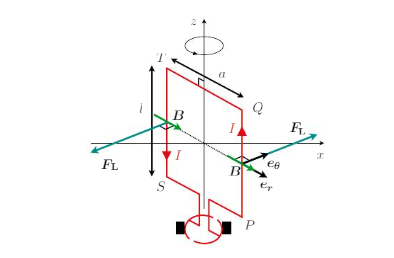
\includegraphics[width=.5\linewidth]{./figures/SchemaPrincipe.png}
	\caption{Schéma de principe extrait du Jolidon}
\end{figure}

\subsubsection*{Couple}

le couple s'obtient en ajoutant le moment subit par les deux branches de la spires soumisent à la force de Laplace:

\begin{equation}
	\mathcal{M} = \int_{M\in[TS]}\vec{OM}\wedge\vec{F_L}(M)+\int_{M\in[PQ]}\vec{OM^\prime}\wedge\vec{F_L}(M^\prime)=IalB\vec{e}_z
\end{equation}

Comme le rotor est constitué de $N$ spires smeblables à celle que nous venons de considérer, on obtient : 

\begin{equation}
	\mathcal{M}_{rotor} = N\mathcal{M} = NialB\vec{e}_z
\end{equation}

Le couple est donc proportionnel au nombre de spires N d'où l'intérêt d'avoir le plus de spires possibles au rotor.\medskip

Le rotor est solidaire d'un arbre de tranmission sur lequel on place une charge à entraîner. Le rotor lui applique un couple $\Gamma$. Discuter du sogne de $\Gamma$ en suivant le Jolidon, permet de décrire le montage expérimental. On établit l'équation mécanique en supposant le référentiel galiléen , théorême du moment cinétique: 

\begin{equation}
	J\dfrac{d\omega}{dt}=-\Gamma-\Gamma_r+NalBI
\end{equation}

On établit l'équation électrique en utilisant la loi des mailles:

\begin{equation}
	U = RI+L\dfrac{dI}{dt}-e_{\rm ext}
\end{equation}

En combinant les équations que l'on a décrit on parvient à un système d'équations:

\begin{equation}
	\left\{
		\begin{array}{cc}
		\Phi\omega & = U-RI-L\dfrac{dI}{dt}\\
		\Gamma & = \Phi I-\Gamma_r-J\dfrac{d\omega}{dt}.
	\end{array}
	\right.
\end{equation}

On a deux équations reliant les quatre variables du quadripôle. En fixant deux d'entre elles on peut déterminer entièrement les variables de fonction du système.

\subsection*{2.4. Caractéristique de fonctionnement}

\subsubsection*{2.4.1. Couple et vitesse de rotation}

En régime permanent de fonctionnement, c'est à dire à $U, I, \Gamma$ et $\omega$ constants le système se réduit à : 

\begin{equation}
	\left\{
		\begin{array}{cc}
		\Phi\omega & = U-RI\\
		\Gamma & = \Phi I-\Gamma_r.
	\end{array}
	\right.
\end{equation}


On voit que les couples de variables mis en jeu sont ($\omega, U$) et ($\Gamma, I$). Le couple est proportionnel à l’intensité i du courant qui circule dans le rotor ($\Gamma = k\Phi$ dans le poly de Phillipe) alors que la vitesse de rotation est pilotée par la tension. Pour un rotor idéal sans pertes joules $R=0$, $\Gamma_r=0$ on aurait même proportionnalité entre $\omega$ et $U$ et $\Gamma$ et $I$.\medskip


Si $i>0$, $\Gamma>0$ la machine fonctionnne en moteur. Si $i<0$ $\Gamma<0$ la machine fonctionne en génératrice.

\subsubsection*{2.4.2. Mesure expérimentale sur un banc d'essai (Poyl TP rennes)}
Poly Phillipe Moteurs - MCC
Réaliser en préparation la mesure de la résistance d'induit pour le moteur et pour la génératrice. On mesure d'abord dans une étude à vide le $\Phi$ dans le moteur avec la génératrice en traçant $E=f(\omega)$
Deuxiemement : étude de charge. On mesure le couple fourni pour une intensité et on trace $\Gamma=f(i)$. Mesure du couple avec une webcam et imageJ. 


\subsection*{2.5. Point de fonctionnement}

La donnée du quadruplet ($U,I, \omega, \Gamma$) est appelée \textbf{point de fonctionnement}  de la machine: il faut donc deux équations supplémentaires pour en déterminer un. Il s'agit de la caractéristique de l'alimentation électrique du rotor généralement de la forme $U = E^\prime-R^\prime I$ ainsi que la caractéristique $\Gamma_c$ de la charge à entraîner. En pratique ces deux nouvelles équations fixent les valeurs de $I$ et $\omega$ vérifiant le système. On peut montrer la caractéristique pour le MCC du Jolidon.

\begin{figure}[ht]
	\centering
  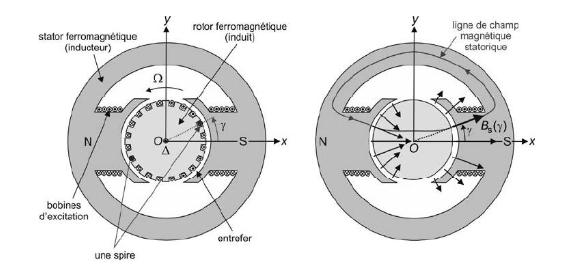
\includegraphics[width=.5\linewidth]{./figures/MCC.png}
	\caption{Caractéristique MCC, extrait du Jolidon}
\end{figure}


\subsection*{2.6. Puissance et rendement (Jolidon)}

Quelque soit son régime de fonctionnement, la MCC consomme de l'énergie dans le stator, en régime moteur, le rotor consomme également une Puissance électrique. Et l'ensemble fournit à la charge mécanique une puissance utile $\Gamma\omega$




\begin{equation}
	\eta_{MCC} = \dfrac{P_{meca}}{P_{elec, stator}+P_{elec,rotor}}
=\dfrac{\Gamma\omega}{UI+U_sI_s}\end{equation}


Le bilan de puissance est déterminé par le système d'equation donné précedemment il suffit de multiplier la premiere equation par I et et $\omega$la deuxieme: 


\begin{equation}
	UI-\Gamma\omega = RI^2+\Gamma_r\omega
\end{equation}

La puissance est dissipe au niveau du rotor, soit par effet joule soit par les pertes mécaniques ($\Gamma_r$). 

Fonctionnement en moteur si $UI>0$ ne donne pas intégrallement la puissance utile $\Gamma\omega>0$ à cause des pertes Joules, mécaniques ainsi que des pertes fer (que l'on a négligé). Fonctionnement en génératrice.

On décrit en suivant le jolidon les différnts types de pertes.

\begin{figure}[ht]
	\centering
	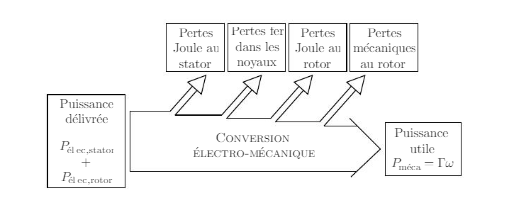
\includegraphics[width=1\linewidth]{./figures/BillanPuissance.png}
	\caption{Bilan de Puissance, extrait jolidon}
\end{figure}

% \section{Machine synchrone}
% On a vu en première année de PTSI le principe d'action d'un champ magnétique tournant sur un moment magnétique. On réalise la mise en pratique d'un moteur.

% \subsection{Structure}
% Dunod PSI 2020 p732-733 et Tec $\&$ Doc 2014 p644, COurs Naval
% La machine synchrone est un exemple de convertisseur électromagnétique réversible, fonctionnant en moteur ou en générateur. Utilisés dans la production d'énergie électrique sous forme de courant alternatif ou bien dans les utilisations de moindre puissance plus courantes comme les véhicules automobiles (Moteur de traction très performant).
% \begin{figure}[ht]
% 	\centering
% 	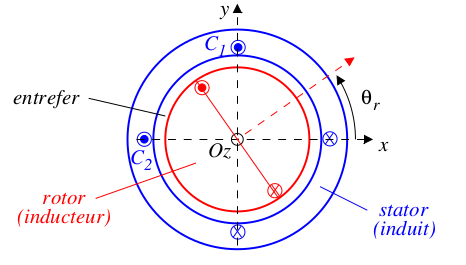
\includegraphics[width=.5\textwidth]{StructureMachinesynchrone.png}
% 	\caption{Schéma cours Naval}
% \end{figure}

% Le matériau constituant le stator (fixe) et le rotor (mobile) est un matériau magnétique linéaire de perméabilité relative infinie. L'épaisseur de l'entrefer est constante. Les deux circuits bobinés sur le stator sont parcourus par un courant sinusoïdal. Le circuit bobiné sur le rotor est parcouru  par un courant permanent. On parle de machine à excitation séparée. L'ensemble du dispositif est de longueur $L$. On cherche à déterminer \vec{B} dans l'entrefer pour en déduire l'énergie magnétique afin de calculer le couple électromagnétique.

% \subsubsection{Stator}
% Partie fixe, alimentés par deux circuits orthogonaux. La machine synchrone est ainsi dite diphasée.
% Champ magnétique tournant avec deux courants sinusoïdaux déphasés de $\pi/2$, voir schéma. (Dunod 2021 PCSI p 877)

% \subsubsection{Rotor}
% Partie ferro tournante, forme variable suivant les applications, rotor à pôle lisses pour de fortes vitesses (entrefer uniforme) cas de l'étude ici.
% Moment magnétique crée avec une spire parcourue par un courant constant.(PCSI 2021 p863 )

% \subsection{Champ dans l'entrefer}

% \subsubsection{Champ crée par une spire}

% Dunod PSI, ligne de champ + contour d'Ampère à dessiner au tableau ou sur transparents. On écrit le théorême d'Ampère, on exprime la circulation dans le Ferro et dans l'entrefer puis comme $\mu_r\ll 1$, on néglige le champ dans le ferro et on en déduit l'expression du champ dans l'entrefer en fonction del'intensité parcourant le fil. Montrer l'allure du champ pour une spire à l'aide d'un programme python ?

% \subsubsection{Répartition spatiale}

% Le champ obtenu avec une seule spire a un défaut majeur : il est discontinu dans l'espace. On cherche à obtenir une répartition angulaire sinusoïdale du champ dans l'entrefer. Si on ajoute d'autres spires avec une répartition spatiale bien choisie, on peut s'approcher d'un champ sinusoïdal (Python ?).

% \subsubsection{Création du champ statorique}
% Il s’agit maintenant de générer à l’aide des deux phases du stator le champ magnétique tournant qui va entraîner le rotor (Cf. principe du moteur synchrone). Deuxième jeu de spires déphasé de $\pi/2$ Calcul dans le Dunod PSI 2020 p 738. On obtient une onde magnétique progressive harmonique qui se propage dans le sens des $\theta$ croissants à la vitesse angulaire $\omega$ ($cos(\theta-\omega t) = f(x-ct)$):
% \begin{equation}
% B_S(\theta,t)=K_SI_S\cos(\theta-\omega t)\vec{u_r}(M).
% \end{equation}


% \subsubsection{Champ rotorique}
% Le rotor tourne en plus d'être parcouru par un courant $i_r$. Sa rotation est repérée par l'angle $\alpha_r$

% Champ magnétique généré par le rotor, rendu spatialement sinusoïdal par la même méthode que pour le champ statorique. $\vec{B}_R(\theta,t)=K_RI_R\cos(\theta-\alpha_r)\vec{u_r}(M)$


% \subsection{Bilan énergétique}

% \subsubsection{Énergie électromagnétique}
% Calcul de l'énergie emmagasinée, DUNOD PSI

% \subsubsection{Couple électromagnétique}
% On reprend la formule donnée dans la première partie et on dérive pour trouver l'expression du couple.
% \begin{equation}
% \Gamma_{em} = \Gamma_{max}\sin{\alpha}.
% \end{equation}
% \begin{Resultat}{Conditions de synchronisme}
% 	La machine synchrone ne développe de couple que si le rotor et le champ glissant statorique tournent à la même vitesse angulaire, ce qui constitue la condition de synchronisme.
% \end{Resultat}


% \subsection{Point de fonctionnement}

% Tracer la sinusoide (Dunod) et commenter.


\section*{Conclusion}

Recap + Interet du moteur à courant continu +machine synchrone

\end{document}

%%
%% FIN DU DOCUMENT
%%
